%
%	Theorieteil
%

\pagebreak
\section{Security Event Stream}

\onehalfspacing

\subsection{Kubernetes Security Signals}

\subsection{SUSE Security}

\subsection{SUSE Security Event Stream}

\begin{figure}[H]
\centering
\caption {SUSE Security Event Stream}
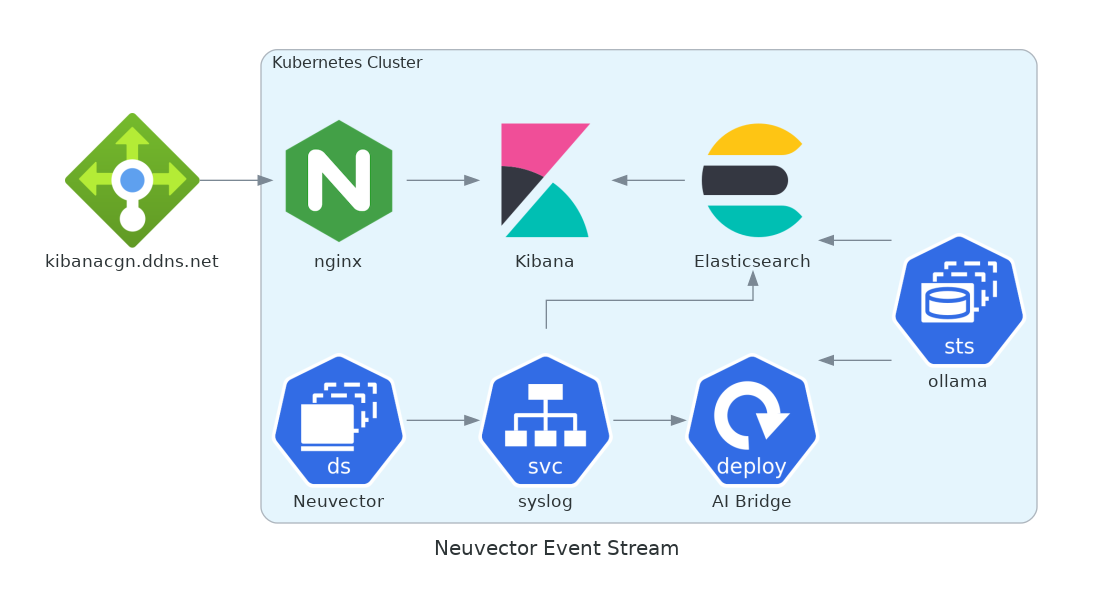
\includegraphics[width=0.9\linewidth]{images/neuvector-event-stream.png}
\label{fig:event-stream}
\end{figure}


\subsection{Experiment setup}

\subsection{Syslog}

\subsection{MQTT}

\subsection{Ollama}

Tool to run LLMs locally.

Self-hosting is not for everyone.\footnote{See \textit{Davies, N. (2026)}: Self-Hosted LLMs in the Real World. \cite{selfHost}}

Several factors should be considered when selecting a local model.\footnote{See \textit{Conway, A. (2026)}: A local LLM for coding. \cite{localModel}}

Ollama is currently embroiled in controversy over license compliance, attribution, and transparency regarding its use of the open-source project llama.cpp. Several voices argue that one should not continue to use Ollama, especially if one prioritizes transparency and performance.\footnote{See \textit{Zetaphor (2025)}: Friends don't let Friends use Ollama. \cite{ollamaDrama}}

Alternatives could be running llama.cpp directly, or exploring other tools such as vLLM or KoboldCPP.

\subsection{Bridge}

\subsection{Elasticsearch}

\subsection{Results}

\begin{lstlisting}[caption=Event Bridge Log, frame=single, basicstyle=\ttfamily, breaklines=true]
You are a helpful Kubernetes security expert
Welcome to the Neuvector event bridge!
meow :3

notification=audit, name=Compliance.ContainerFile.Violation, level=Warning, reported_timestamp=1775940060, reported_at=2026-04-11T20:41:00Z, cluster_name=aks-893050, enforcer_name=neuvector-enforcer-pod-p4dr5, workload_name=cattle-cluster-agent-74cb77b56c-85v9w, workload_domain=cattle-system, workload_image=docker.io/rancher/rancher-agent:v2.12.3, workload_service=cattle-cluster-agent.cattle-system, critical_vul_cnt=0, high_vul_cnt=0, medium_vul_cnt=0, message=, items=[D.4.8 WARN - Total 2 files have setgid mode D.4.8 WARN - Total 13 files have setuid mode]
 
\end{lstlisting}

\subsection{Software Versions}

In the experiment, the following open-source software versions were used.

\begin{table}[ht]
  \caption{Software Versions}
    \begin{tabular}{| l | l |}
    \hline
    Software & Version \\
    \hline\hline
    Elasticsearch & 8.19.3 \\
    \hline
    Kubernetes (AKS) & 1.33.8 \\
    \hline
    MCP-Server & 0.0.60 \\
    \hline
    Mosquitto & 2.0.22 \\
    \hline
    NeuVector & 5.4.9 \\
    \hline
    Ollama & 0.14.2 \\
    \hline
    Rancher & 2.12.3 \\
    \hline
    Syslog-ng & 4.10.2 \\
    \hline
    \end{tabular}%
  \label{tab:aksBenchmark}%
\end{table}%

Some of the versions above are likely superseded.

\subsection{MCP Server}

\begin{figure}[H]
\centering
\caption {MCP Server}
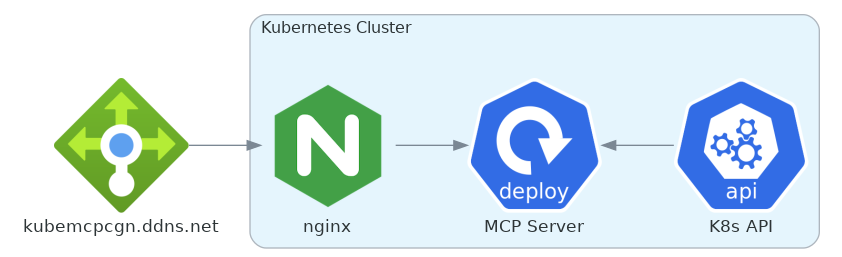
\includegraphics[width=0.9\linewidth]{images/mcp-server.png}
\label{fig:mcp-server}
\end{figure}

\subsection{Air Gap}

After training, model knowledge quickly becomes outdated.

As discussed in \ref{threat-intelligence}, it's important to amend the model knowledge with current information.

Another factor to consider is model bias.\footnote{See \textit{Xu, J. et al. (2026)}: AI self preference. \cite{xu2026}}

\subsection{GDPR}
